% Story check of the GT2027 paper: outline-only mode of the academic-paper skill (structure architect format),
% evidence map and story-drift assessment. Build: pdflatex story_check.tex (twice). The word-budget figure is
% drawn by word_budget.py in this folder (python3 -I word_budget.py), which also writes word_budget.txt.
\documentclass[10pt]{article}
\usepackage[utf8]{inputenc}
\usepackage[T1]{fontenc}
\usepackage{lmodern}
\usepackage{textcomp}
\usepackage[a4paper,margin=17mm]{geometry}
\usepackage{amsmath,amssymb}
\usepackage{booktabs,array,longtable,tabularx,graphicx,enumitem,float}
\usepackage[dvipsnames]{xcolor}
\usepackage{tikz}
\usetikzlibrary{positioning,arrows.meta,fit}
\usepackage[colorlinks=true,linkcolor=MidnightBlue,urlcolor=MidnightBlue]{hyperref}
\setlength{\parskip}{4pt}
\setlength{\parindent}{0pt}
\setlist{itemsep=1pt,topsep=2pt}
\setlength{\emergencystretch}{2em}
\renewcommand{\arraystretch}{1.15}
\setlength{\tabcolsep}{3pt}
\graphicspath{{../../figures/}{./}}
\newcolumntype{L}[1]{>{\raggedright\arraybackslash}p{#1}}
\newcommand{\st}[1]{\textsf{\small #1}}
% status colours (Okabe-Ito)
\definecolor{oiBlue}{HTML}{0072B2}\definecolor{oiOrange}{HTML}{E69F00}\definecolor{oiGreen}{HTML}{009E73}
\definecolor{oiVerm}{HTML}{D55E00}\definecolor{oiSky}{HTML}{56B4E9}\definecolor{oiPink}{HTML}{CC79A7}

\title{GT2027 paper: story check, outline and evidence map}
\author{}
\date{27 November 2026}

\begin{document}
\maketitle
\vspace{-12mm}

{\small Inputs read: \texttt{CLAUDE.md}; \texttt{WRITING\_STYLE.md}; the structure-architect agent and the
outline-only entry of the academic-paper skill (v3.24.4); \texttt{planning/writeup\_plan.tex} in two states, the
committed plan of record (HEAD \texttt{6fa3e15}, 27 Nov 04:10) and the working copy (uncommitted, edited today);
\texttt{manuscript/main\_claude.tex} and its PDF (18 pages, 27 Nov 20:34); \texttt{planning/tracking.md};
\texttt{figures/code/data/*.txt}; \texttt{planning/maths\_audit/crvp\_upwash/crvp\_upwash\_literature.md} and
\texttt{compensating\_errors/compensating\_errors\_literature.md}. \texttt{planning/log.md} does not exist.
The swap test and the lateral budget below were passed on by the coordinator with numbers; their files lie under
\texttt{/mnt} and were not opened, so those numbers are quoted as received and are not in the plan or the
manuscript.}

%=====================================================================================================
\section*{A\quad Verdict}

\begin{center}
\fbox{\parbox{0.94\textwidth}{\vspace{2pt}
\textbf{Partly shifted.} The spine of the plan is intact: the scale-resolving rungs agree in $\bar\eta$ from 20M
points, the mesh-independent RANS is 29--33\,\% low with a narrow film and a laminar mid-pitch layer, the RANS error
is attributed to the closure inputs in three steps, and the a posteriori runs show that a $\Pr_t$ setting fixes
the centreline and not the spread. Two links of the chain have moved.

\textbf{Most important change.} The explanation of the narrow RANS film has moved part of its weight from the
closure to the mean flow. In the plan of record the RANS $\mu_t$ was 0.4--0.7 of the reference throughout the jet
and film, and the narrow film followed from weak turbulent diffusion. In the manuscript the deficit is confined to
a near-wall layer below $z_x(x)$ (0.55--0.66 of the reference), the eddy viscosity above it matches through
compensating factors, and Section 4.1 adds a mean-flow route: a stronger counter-rotating vortex pair (CRVP) and a
mean upwash flux several times the reference. The new swap test and lateral budget (not yet in the paper) support
the mean-flow route downstream of $x/D\sim10$, while Section 4.2 still states that the narrow film is the result of
weak lateral diffusivity. The paper now carries two explanations of one effect without stating how they combine.

\textbf{Second change.} Aim 4 (resolution needed) is thinner than planned: Section 3.3 lacks its numbers (open
marker), its figure is stale (four meshes, far film labelled 10--25), and one sentence of it contradicts the
figure.
\vspace{2pt}}}
\end{center}

\textbf{Claims ahead of the evidence} (details in E):
\begin{enumerate}[label=\arabic*.]
\item ``A stronger CRVP \dots\ keeps the coolant on the centreline and sweeps hot gas under the flanks'' (4.1) and
  ``consistent with its stronger CRVP'': the flux excess is now measured to come from both the RANS velocity field
  and the RANS coolant distribution; the vortex pair itself has not been isolated.
\item ``The narrow, steep film of the RANS is thus the result of its weak lateral diffusivity'' (4.2): in conflict
  with the new lateral budget, which shows the RANS outward turbulent flux equal to the reference from $x/D\sim10$.
\item ``The RANS turbulent flux is about half that of the reference'': the ratio depends on the height of the
  surface (scratch test at fixed heights: 0.67--0.98 at $z/D=1.0$, negative at $z/D$ 0.25 and partly at 0.5); only
  the ordering of the two parts is robust.
\item ``0.55--0.75'' for the near-wall $\mu$ ratio in the body (macro \texttt{\textbackslash muNearHigh}): the data
  table and the abstract give 0.55--0.66.
\item ``The 20M LES and the 50M 3DNS lie $\sim$10\,\% above the reference'' (eddy viscosity): no data file found;
  the plan of record stated the opposite (within $\pm2$ SE of zero); due from W1 item 3 on 1 Dec.
\end{enumerate}

\newpage
%=====================================================================================================
\section*{B\quad Story chain, plan against manuscript}

Plan of record: committed \texttt{writeup\_plan.tex} (HEAD, 27 Nov 04:10). The working copy of the plan was
edited today and already carries most manuscript changes; where it differs from the manuscript this is listed in
E3. Status: \st{unchanged}, \st{sharpened}, \st{changed}, \st{dropped}, \st{new}.

{\footnotesize
\begin{longtable}{@{}L{1.5cm} L{4.8cm} L{5.0cm} L{1.5cm} L{3.9cm}@{}}
\toprule
Section & Plan of record & Manuscript now & Status & Reason \\
\midrule
\endhead
Intro & RANS errors known by place, not by share; no study splits the error by cause and region; no single
mesh family from RANS to DNS; laminar approach layer relevant to small cores. & Same chain, nine paragraphs.
Literature value of the best-practice RANS $\bar\eta$ error missing (open marker). & \st{unchanged} & Gap
statement still names the closure only; it does not prepare the mean-flow (CRVP) finding of 4.1. \\
Aims & 1 error per rung; 2 attribution to $\mu_t$ factors, $\Pr_t$, spanwise; 3 a posteriori incl.\ $\gamma=1$;
4 resolution (supporting). & Same four aims. & \st{unchanged} & Aim 3 depends on an unfinished run; aim 4 is
answered by $\bar\eta$ agreement, not by the resolution numbers. \\
Methods & Configuration, mesh family, $\Delta/\eta_K$ per region with numbers, five meshes. & Text present;
numbers of 3.3 missing; figure with four meshes; mesh-class figure F2 not used. & \st{unchanged} (incomplete) &
Three open markers in Methods. \\
4.1 hole & BR spread from diffuser recovery; RANS +4.7\,\%; bubble coherence (F6). & Same; F6 not used, coherence
in text only. & \st{unchanged} & Figure cut for length. \\
4.1 mean flow & CRVP 1.2--1.8 times stronger, lower; WV kept to $x/D$ 15 in 193M, lost by 5 in RANS; flux split
``ratios to be confirmed''. & Same, with the flux through the final $z_x$; ``about half'' and ``several times'';
cause stated as the stronger CRVP. & \st{sharpened} & Flux surface fixed to $z_x$; ratios in a comment only
(0.37--0.61 and 1.65--5.9). \\
4.1 wall layer & Laminar RANS mid-pitch; one $\gamma$ definition; spread transition between the jets. & Same;
wall-state figure F9 not used, its numbers in text. & \st{unchanged} & One intermittency definition used in both
plan and manuscript (verified). \\
4.1 $\eta$ & SR rungs within 0.008; RANS 29--33\,\% low; distribution error; mid-pitch gap from laminar
approach. & Same; the $\gamma>0.8$ comparison with the experiment removed (open marker). & \st{unchanged} & Stale
numbers removed. \\
4.2 $\mu_t$ & RANS $\mu_t$ 0.4--0.7 of the reference in jet and film (strain$^2$-weighted regional least
squares, $z/D\ge0.3$); aligned length the largest term. & Below $z_x$: 0.55--0.66 (body says 0.55--0.75); length
largest deficit, alignment gives part back. Above $z_x$: close to one through compensating $k^{1/2}$, length and
alignment. & \st{changed} & New estimator (3D strain mask, conditional span means), new layer definition; the
interim far-wall over-prediction was an averaging artefact (E1). \\
4.2 $\Pr_t$ & 0.30 / 0.23 / 0.47 (jet, near, far film to $x/D$ 25). & 0.30 / 0.23 / 0.45, SE $\le$0.013. &
\st{sharpened} & Far film cut to $x/D$ 20; volume values with jackknife SE. \\
4.2 spanwise & $\alpha_y/\alpha_z$ 3.2 and 1.7 on the flanks; RANS lateral diffusivity about half, mostly the
$\Pr_t$ setting; narrow film from weak lateral diffusivity. & Same. & \st{unchanged} & Now in tension with the
lateral budget (E2). \\
4.3 & $\Pr_t$ sweep saturates at 36--48\,\%; QCR 72\,\%; QCR+$\Pr_t$ 0.4 97\,\% with the wrong shape; film-only
heat flux closest; three runs pending. & Same; two recovered shares added (63\,\%, 54\,\%) by the drafting
session; three runs still pending. & \st{unchanged} (incomplete) & Shares computed from window means, not in the
plan. \\
Abstract & Not in the plan. & Rewritten 26 Nov; omits the CRVP/upwash finding and the film-only heat-flux
result. & \st{new} & Abstract and conclusions do not carry the same findings. \\
Conclusions & ``Mirror the aims''; no content. & Four outcomes; item 1 adds ``moves coolant off the wall by mean
upwash where the reference moves it by turbulence''. & \st{new} & First statement of the mean-flow mechanism as a
headline. \\
\bottomrule
\end{longtable}}

\begin{figure}[H]
\centering
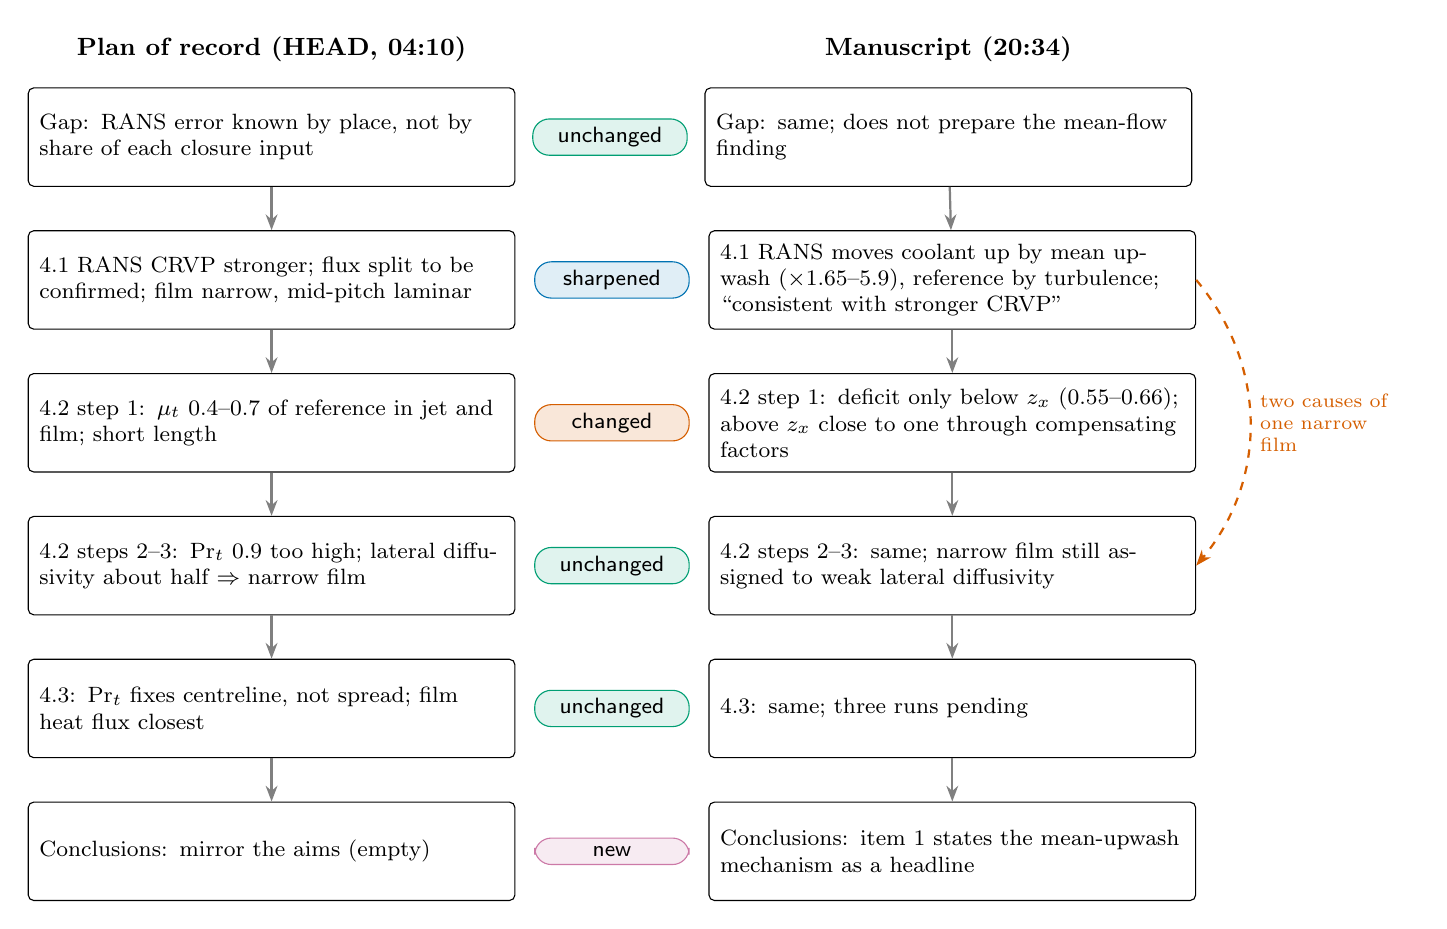
\begin{tikzpicture}[
  every node/.style={font=\footnotesize, align=left},
  box/.style={draw, rounded corners=2pt, text width=5.9cm, inner sep=4pt, minimum height=1.25cm},
  stat/.style={draw, rounded corners=6pt, text width=1.75cm, align=center, inner sep=3pt, font=\footnotesize\sffamily},
  arr/.style={-{Stealth[length=2mm]}, thick, gray},
  node distance=0.55cm and 0.35cm]
% left column
\node[box] (l1) {Gap: RANS error known by place, not by share of each closure input};
\node[box, below=of l1] (l2) {4.1 RANS CRVP stronger; flux split to be confirmed; film narrow, mid-pitch laminar};
\node[box, below=of l2] (l3) {4.2 step 1: $\mu_t$ 0.4--0.7 of reference in jet and film; short length};
\node[box, below=of l3] (l4) {4.2 steps 2--3: $\Pr_t$ 0.9 too high; lateral diffusivity about half $\Rightarrow$ narrow film};
\node[box, below=of l4] (l5) {4.3: $\Pr_t$ fixes centreline, not spread; film heat flux closest};
\node[box, below=of l5] (l6) {Conclusions: mirror the aims (empty)};
% right column
\node[box, right=2.4cm of l1] (r1) {Gap: same; does not prepare the mean-flow finding};
\node[font=\small\bfseries, above=0.2cm of l1] {Plan of record (HEAD, 04:10)};
\node[font=\small\bfseries, above=0.2cm of r1] {Manuscript (20:34)};
\node[box, right=2.45cm of l2] (r2) {4.1 RANS moves coolant up by mean upwash ($\times$1.65--5.9), reference by turbulence; ``consistent with stronger CRVP''};
\node[box, right=2.45cm of l3] (r3) {4.2 step 1: deficit only below $z_x$ (0.55--0.66); above $z_x$ close to one through compensating factors};
\node[box, right=2.45cm of l4] (r4) {4.2 steps 2--3: same; narrow film still assigned to weak lateral diffusivity};
\node[box, right=2.45cm of l5] (r5) {4.3: same; three runs pending};
\node[box, right=2.45cm of l6] (r6) {Conclusions: item 1 states the mean-upwash mechanism as a headline};
\foreach \a/\b in {l1/l2,l2/l3,l3/l4,l4/l5,l5/l6,r1/r2,r2/r3,r3/r4,r4/r5,r5/r6} \draw[arr] (\a) -- (\b);
% status nodes in the middle
\path (l1.east) -- (r1.west) node[midway, stat, draw=oiGreen, fill=oiGreen!12] {unchanged};
\path (l2.east) -- (r2.west) node[midway, stat, draw=oiBlue, fill=oiBlue!12] {sharpened};
\path (l3.east) -- (r3.west) node[midway, stat, draw=oiVerm, fill=oiVerm!15] {changed};
\path (l4.east) -- (r4.west) node[midway, stat, draw=oiGreen, fill=oiGreen!12] {unchanged};
\path (l5.east) -- (r5.west) node[midway, stat, draw=oiGreen, fill=oiGreen!12] {unchanged};
\path (l6.east) -- (r6.west) node[midway, stat, draw=oiPink, fill=oiPink!15] {new};
% tension
\draw[-{Stealth[length=2mm]}, thick, oiVerm, dashed] (r2.east) to[bend left=40] node[right, font=\scriptsize, text width=1.9cm, text=oiVerm] {two causes of one narrow film} (r4.east);
\end{tikzpicture}
\caption{Claim chain. Left: plan of record. Right: manuscript. Middle: status of each link. Dashed: the narrow
RANS film is explained by the mean flow in 4.1 and by the lateral diffusivity in 4.2, without a statement of how
the two combine.}
\end{figure}

\newpage
%=====================================================================================================
\section*{C\quad Detailed outline of the paper as it stands}

\textbf{Structure pattern:} Conference paper (pattern 6), IMRaD with literature inside the Introduction; the
GPPS-paper order of the style guide (Introduction, Research Aims, Methods, Results and Discussion, Conclusions).

\textbf{Overview.} The paper narrows from shaped-hole design by RANS to a test bed in which only model and mesh
change (7-7-7 hole, flat plate, laminar approach layer, one mesh family from 5M to 193M). It shows that every
scale-resolving rung predicts $\bar\eta$ and that the RANS film is narrow, then follows the coolant from the hole
to the wall (4.1), breaks the RANS mixing error into closure inputs (4.2) and tests corrections (4.3).

\textbf{Review criteria coverage:} \texttt{criteria\_binding\_unavailable}; no venue-alignment claim is made.

\textbf{Word budget.} Target 15 pages in asmeconf against 18 now. Assumption: words scale with pages at the
present figure count (16 figures, 2 tables), so the body budget is $7642\times15/18\approx6370$ words, shared by
judgement (Figure~\ref{fig:wb}; \texttt{word\_budget.py}). A 1270-word cut alone may not reach 15 pages if two
full-width figures stay; dropping one full-width figure is worth about $\frac{1}{3}$ page.

\begin{figure}[H]
\centering
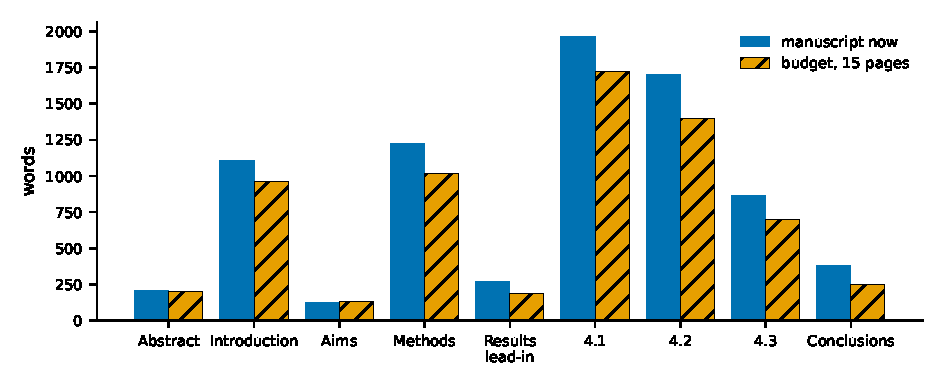
\includegraphics[width=0.78\textwidth]{word_budget.pdf}
\caption{Words per block of \texttt{main\_claude.tex} (blue) against the 15-page budget (orange, hatched).
Counted by \texttt{word\_budget.py}: comments, equations, tables and figure environments excluded; inline maths
counted as one word.}\label{fig:wb}
\end{figure}

{\footnotesize
\begin{longtable}{@{}L{2.2cm} L{8.4cm} L{3.4cm} L{2.4cm}@{}}
\toprule
Section & Paragraph block: claim & Carried by & Words now / budget \\
\midrule
\endhead
\multicolumn{4}{@{}p{16.4cm}@{}}{\textbf{1 Introduction.} Purpose: narrow from design practice to the gap and justify the
configuration. Sources: the reference list of plan P1--P8.} \\
 & P1 RANS remains the design tool; its accuracy sets the design. Literature value of the RANS $\bar\eta$ error
missing. & Bogard \& Thole; Milani & 1107 / 960 (section) \\
 & P2 7-7-7 is the most documented shaped hole. & Schroeder \& Thole; Haydt & \\
 & P3 Flat plate at zero pressure gradient isolates model and resolution. & Saumweber; Oliver; Bin \& Yang & \\
 & P4 RANS errors traced to Eq.~1 (Boussinesq) and Eq.~2 (GDH); gap: no split by cause. & Acharya; Stratton \&
Shih; Ling & \\
 & P5a Mean features; RANS--resolved match not reported. & Fric \& Roshko; Thole & \\
 & P5b Instantaneous features; at VR $\sim$1 mixing is broadband. & Fawcett; Tyagi \& Acharya & \\
 & P6 Scale-resolving studies differ in model, mesh and measure at once. & Peet \& Lele; Oliver; Bin \& Yang & \\
 & P7--P8 Laminar approach layer; the test bed. & Clark; Kar; Goldstein \& Yoshida & \\
\multicolumn{4}{@{}p{16.4cm}@{}}{\emph{Transition:} the gap is stated; the aims follow. \emph{Cut:} P5b and P6 to two
sentences each (about 150 words).} \\
\midrule
\textbf{2 Aims} & Four numbered aims; conclusions mirror them. & none & 128 / 130 \\
\midrule
\multicolumn{4}{@{}p{16.4cm}@{}}{\textbf{3 Methods.} Purpose: let the reader place every rung, boundary and region.} \\
3.1 Configuration & Geometry, operating point (Eq.~3--4), solvers, BC, eight regions. & Fig.~1, Table~1 &
1222 / 1020 (section) \\
3.2 Mesh family & Coarsening by $s$ (Eq.~5--6); seven classes depart. & text only (F2 dropped) & \\
3.3 Resolution & $\Delta/\eta_{K,193}\le2$; diffuser least resolved. Numbers missing; one sentence contradicts the
figure (E2). & Fig.~2 (stale) & \\
\multicolumn{4}{@{}p{16.4cm}@{}}{\emph{Transition:} 193M b010 is the reference. \emph{Cut:} BC paragraph and the 3DNS
filter detail (about 150 words).} \\
\midrule
Results lead-in & Flow-to-closure order; 6 against 10 FT; Fig.~3 names CRVP, HV, WV. & Fig.~3 & 273 / 190 \\
\midrule
\multicolumn{4}{@{}p{16.4cm}@{}}{\textbf{4.1 Coolant flow.} Purpose: follow the coolant from hole to wall; locate the RANS
error in the mean flow and the wall layer.} \\
The hole & Diffuser separation sets BR; RANS +4.7\,\% is a model effect; set aside. & Fig.~4, Table~1 &
1964 / 1720 (section) \\
Jet above wall & CRVP 1.2--1.8 times stronger, 0.1$D$ lower; WV lost by $x/D$ 5; vertical flux through $z_x$:
turbulent $>$ mean flow from $x/D$ 4.3 in the 193M, never in the RANS; plume 0.75 wide, $\bar\eta$ 0.67, centreline
1.29 at $x/D$ 20. & Fig.~5, Fig.~6 (two-part) & \\
Layer between jets & One $\gamma$ definition; RANS mid-pitch laminar to $x/D$ 20; 193M and LES $\gamma$ within
0.03; coherent share 0.05--0.08. & Fig.~7, Fig.~8 & \\
Effectiveness & SR rungs within 0.008; RANS 29--33\,\% low; distribution error; mid-pitch gap from the laminar
approach layer. & Fig.~9 & \\
\multicolumn{4}{@{}p{16.4cm}@{}}{\emph{Transition:} ``From the flow to the closure'' defines $\mu_{\mathrm{eff}}$ (Eq.~8) and
classic $\Pr_t$ (Eq.~9--10). \emph{Cut:} the bubble-coherence and BR-sensitivity sentences.} \\
\midrule
\multicolumn{4}{@{}p{16.4cm}@{}}{\textbf{4.2 Breakdown.} Purpose: compare the two inputs of the RANS heat flux with the
reference.} \\
Eddy viscosity & Factor form (Eq.~11) and exact log split (Eq.~12); 3D strain mask; $z_x$; below $z_x$ 0.55--0.66
(length largest); above $z_x$ close to one through compensating factors; model not mesh. & Fig.~10 maps, Fig.~11
split, Fig.~12 planes & 1705 / 1400 (section) \\
$\Pr_t$ & Map and regional values 0.30 / 0.23 / 0.45 against 0.9. & Fig.~13, Fig.~14 & \\
Spanwise & $\alpha_y/\alpha_z$ 3.2, 1.7; RANS lateral diffusivity 0.5--0.6, mostly $\Pr_t$ setting. & Fig.~15 & \\
Remedies & One remedy per factor; all factors in error. & none & \\
\multicolumn{4}{@{}p{16.4cm}@{}}{\emph{Transition:} which remedy recovers $\bar\eta$. \emph{Cut:} Fig.~12 text (planes) to
three sentences; remedies to four lines.} \\
\midrule
\multicolumn{4}{@{}p{16.4cm}@{}}{\textbf{4.3 A posteriori.} Purpose: change one input at a time; amount and shape.} \\
Method, $\Pr_t$, heat flux, stress, limits & $\Pr_t$ saturates at 36--48\,\%; QCR 72\,\% and worse centreline;
film-only heat flux closest in shape; three runs pending. & Table~2, Fig.~16 & 865 / 700 \\
\midrule
\textbf{5 Conclusions} & Four outcomes mirroring the aims. & none & 378 / 250 \\
\bottomrule
\end{longtable}}

\newpage
%=====================================================================================================
\section*{D\quad Evidence map: abstract and conclusions}

Strength: \textbf{M} measured (number read from a data file or figure of this project), \textbf{I} inferred
(interpretation of measured numbers), \textbf{N} not yet shown. Data source abbreviations: \texttt{d/} =
\texttt{figures/code/data/}; ``fig'' = the paper figure itself; ``coord.'' = numbers received from the coordinator,
files not opened.

{\footnotesize
\begin{longtable}{@{}L{0.5cm} L{4.9cm} L{2.0cm} L{4.0cm} L{0.5cm} L{4.4cm}@{}}
\toprule
\# & Claim & Figure / table & Data source & Str. & Gap \\
\midrule
\endhead
\multicolumn{6}{@{}l}{\textbf{Abstract}} \\
A1 & Where closure assumptions fail is known; the share each carries is not. & Intro P4 & literature & I & No
search note checks ``share''; acceptable as framing. \\
A2 & From 20M points upward $\bar\eta$ within 0.008 of the 193M. & Fig.~9a & window means (plan 4.1 iv) & M &
None. \\
A3 & RANS mesh-independent, 29--33\,\% low beyond $x/D$ 7, narrow film, laminar mid-pitch. & Fig.~9, Fig.~7, 8 &
plan 4.1 iv; RANS 5M/50M & M & None. \\
A4 & Near the wall RANS $\mu$ is a half to two thirds of the reference, mostly short length. & Fig.~10d, 11 &
\texttt{d/meff\_maps\_table.txt} (slabs: $\ln$ $-0.42$ to $-0.59$) & M & Body text says 0.55--0.75; layer defined
by the ratio itself (E1). \\
A5 & Above that layer close to the reference through compensating errors. & Fig.~10 & same file (slabs
1.01--1.11; band 0.98--1.03) & M/I & Only 32--56\,\% of the volume above $z_x$ passes the mask; ``compensating'' is
a reading. \\
A6 & $\Pr_t$ 0.30 jet, 0.23--0.45 film, against 0.9. & Fig.~14 & \texttt{d/prt\_volume\_se.txt} & M & None. \\
A7 & RANS lateral heat diffusivity 0.5--0.6 at the film edges, mostly the $\Pr_t$ setting. & Fig.~15b &
plan F19 split (no data file in \texttt{d/}) & M & Confidence medium (edge definition, RANS gradients). \\
A8 & Lowering $\Pr_t$ corrects the centreline, not the spread. & Table~2, Fig.~16 &
\texttt{d/aposteriori\_table.txt} & M & None. \\
A9 & (missing) CRVP and upwash finding of 4.1. & Fig.~6 & -- & -- & Abstract omits the 4.1 headline that
conclusion 1 carries. \\
A10 & (missing) film-only heat-flux run, closest in shape. & Table~2 & -- & -- & Abstract omits the 4.3
headline that conclusion 3 carries. \\
\midrule
\multicolumn{6}{@{}l}{\textbf{Conclusions}} \\
C1a & SR rungs within 0.008 and with the experiment. & Fig.~9 & plan 4.1 iv & M & Holds for $\bar\eta$; mid-pitch
$\eta$ disagrees with the experiment (stated in 4.1). \\
C1b & RANS CRVP stronger and lower. & Fig.~6 top & \texttt{d/mean\_features\_table.txt} (smoothed volumes: $\Gamma$ ratio 1.06--1.76 at $x/D$ 2--20; $z_c$ ratio 0.83--0.98 at $x/D$ 4--20) & M & Text
values (1.8 at $x/D$ 3, 1.2 at 20) come from the fine cross-planes; the volume table gives 1.06 at $x/D$ 15 (0.97
with the 0.4 contour). Two sources; the paper should name one. \\
C1c & Turbulent flux about half, mean upwash flux several times; RANS moves coolant up by upwash, reference by
turbulence. & Fig.~6 bottom-a & n7 surface file (\texttt{/mnt}, via \texttt{fig\_flux\_eta.py}); ratios in a
\texttt{.tex} comment & M & Ordering holds at $z/D$ 0.25, 0.5, 1.0 (scratch test; 193M crossover at $x/D$ 8, 5,
3); the ratio does not: turbulent RANS/193M 0.67--0.98 at $z/D=1.0$, negative lower down. \\
C1d & (implied by 4.1) stronger CRVP causes the excess upwash and the centreline concentration. & Fig.~6 & coord.:
swap test, lateral budget & I & Swap test: velocity effect 1.2--2.9$\times$, coolant-distribution effect
1.6--2.7$\times$; CRVP not isolated. Not in plan or manuscript. \\
C1e & RANS layer between jets laminar; reference turbulent over $x/D$ 10--15. & Fig.~7, 8 & intermittency
policy (\texttt{maths\_audit/intermittency}) & M & None. \\
C2a & Near-wall layer 0.62--0.94$D$; RANS $\mu$ half to two thirds; length largest, energy low, alignment offsets.
& Fig.~10, 11 & \texttt{d/meff\_maps\_table.txt}, \texttt{d/near\_wall\_boundary\_zx.txt} & M & Note in the table:
split layer taken to the ``full-pitch'' $z_x$, the map line to the point-file $z_x$; same values to be confirmed. \\
C2b & Above the layer close through compensating errors. & Fig.~10 & same & M/I & As A5; manual grey mask at the
jet edge not disclosed in the caption (E4). \\
C2c & $\Pr_t$ 0.23--0.45 in the film. & Fig.~14 & \texttt{d/prt\_volume\_se.txt} & M & None. \\
C2d & Lateral heat diffusivity 0.5--0.6, mostly $\Pr_t$. & Fig.~15 & plan F19 & M & At $x/D$ 10 the $\mu_t$ term is
$+0.91$ (RANS higher than the classic 193M viscosity), not discussed against C2a. \\
C3a & Lower $\Pr_t$ recovers 36--48\,\%, fixes centreline not spread. & Table~2 & \texttt{d/aposteriori\_table.txt}
& M & None. \\
C3b & QCR 72\,\%, worsens centreline. & Table~2 & same & M & None. \\
C3c & Film heat flux, RANS mean flow unchanged, closest in shape. & Table~2, Fig.~16 & same & M & Recovered share
63\,\% computed in the drafting pass, not in the plan. \\
C3d & Stress and laminar mid-pitch runs to come. & -- & -- & N & Three runs pending. \\
C4a & Diffuser least resolved on every mesh. & Fig.~2a & \texttt{fig\_resolution.py} & M & Figure has four
meshes; plan has five. \\
C4b & A 20M LES of this family predicts $\bar\eta$ within 0.008. & Fig.~9 & as A2 & M & Resolution numbers of
3.3 missing, so ``resolution needed'' (aim 4) is answered only by the outcome. \\
\bottomrule
\end{longtable}}

\newpage
%=====================================================================================================
\section*{E\quad Story-drift assessment}

\subsection*{E1\quad What shifted and why}

\textbf{Eddy viscosity (4.2, step 1).} Three states in three days.
\begin{enumerate}[label=(\roman*)]
\item Plan of record: regional least-squares $\mu_R$, strain$^2$-weighted, $z/D\ge0.3$. RANS 0.4--0.7 of the
  reference in the film; aligned length the largest term. The estimator put 91--96\,\% of the weight below
  $z/D=0.3$, which the cut removed (\texttt{maths\_audit/estimator/estimator.md}).
\item Interim (recorded as ``previous definition'' in \texttt{d/meff\_maps\_table.txt}): near-wall lower bands
  0.56--0.61, upper bands 1.9--2.5 and far-wall bands 4.4--4.8 (22.3 unmasked). Read as near-wall under-prediction
  and far-wall over-prediction.
\item Now: a 3D mask $|S^*|D/U_\infty>0.05$ applied before the span average. Masked volume-weighted medians of the
  far-wall bands fall to 1.12--1.17; unfiltered they are 8--16. The over-prediction came from points without mean
  strain, where $\mu_{\mathrm{eff}}$ is not defined. Verified from the file.
\end{enumerate}
Reason for the shift: an estimator choice with a physical justification (an eddy viscosity needs strain), stated
in the manuscript. Two consequences are not stated in the manuscript. First, $z_x$ is defined as the height where
the ratio first reaches one, so ``lower below $z_x$'' holds by construction; the findings are the size of the
deficit and the factor pattern, not its sign. Second, above $z_x$ only 32--56\,\% of the volume passes the mask
(``kept'' column, slabs at $x/D$ 5--20), so ``close to one'' describes the strained part only, while the RANS
heat flux acts wherever a temperature gradient exists.

\textbf{Mean flow (4.1).} New since the plan of record: the vertical coolant flux through $z_x$, split into mean
flow and turbulent parts. The figure (below, left) shows the reference turbulent flux above its mean-flow flux
from $x/D\sim4.3$ and the RANS mean-flow flux above its turbulent flux everywhere. This moves part of the
explanation of the narrow film from the closure to the mean flow.

\begin{figure}[H]
\centering
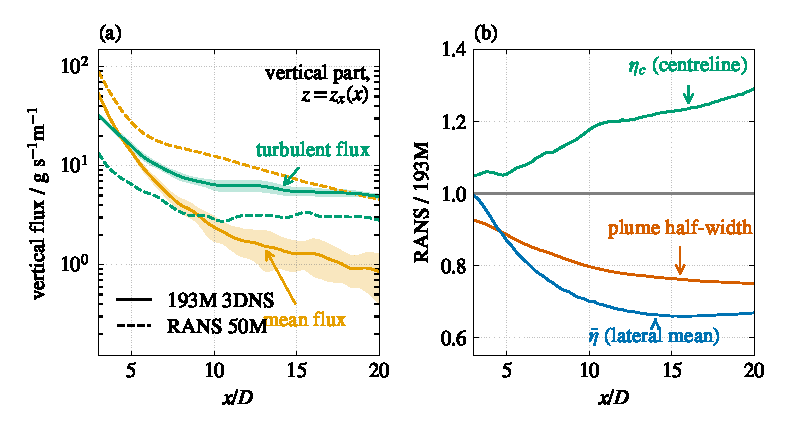
\includegraphics[width=0.56\textwidth]{fig_flux_eta.pdf}\hfill
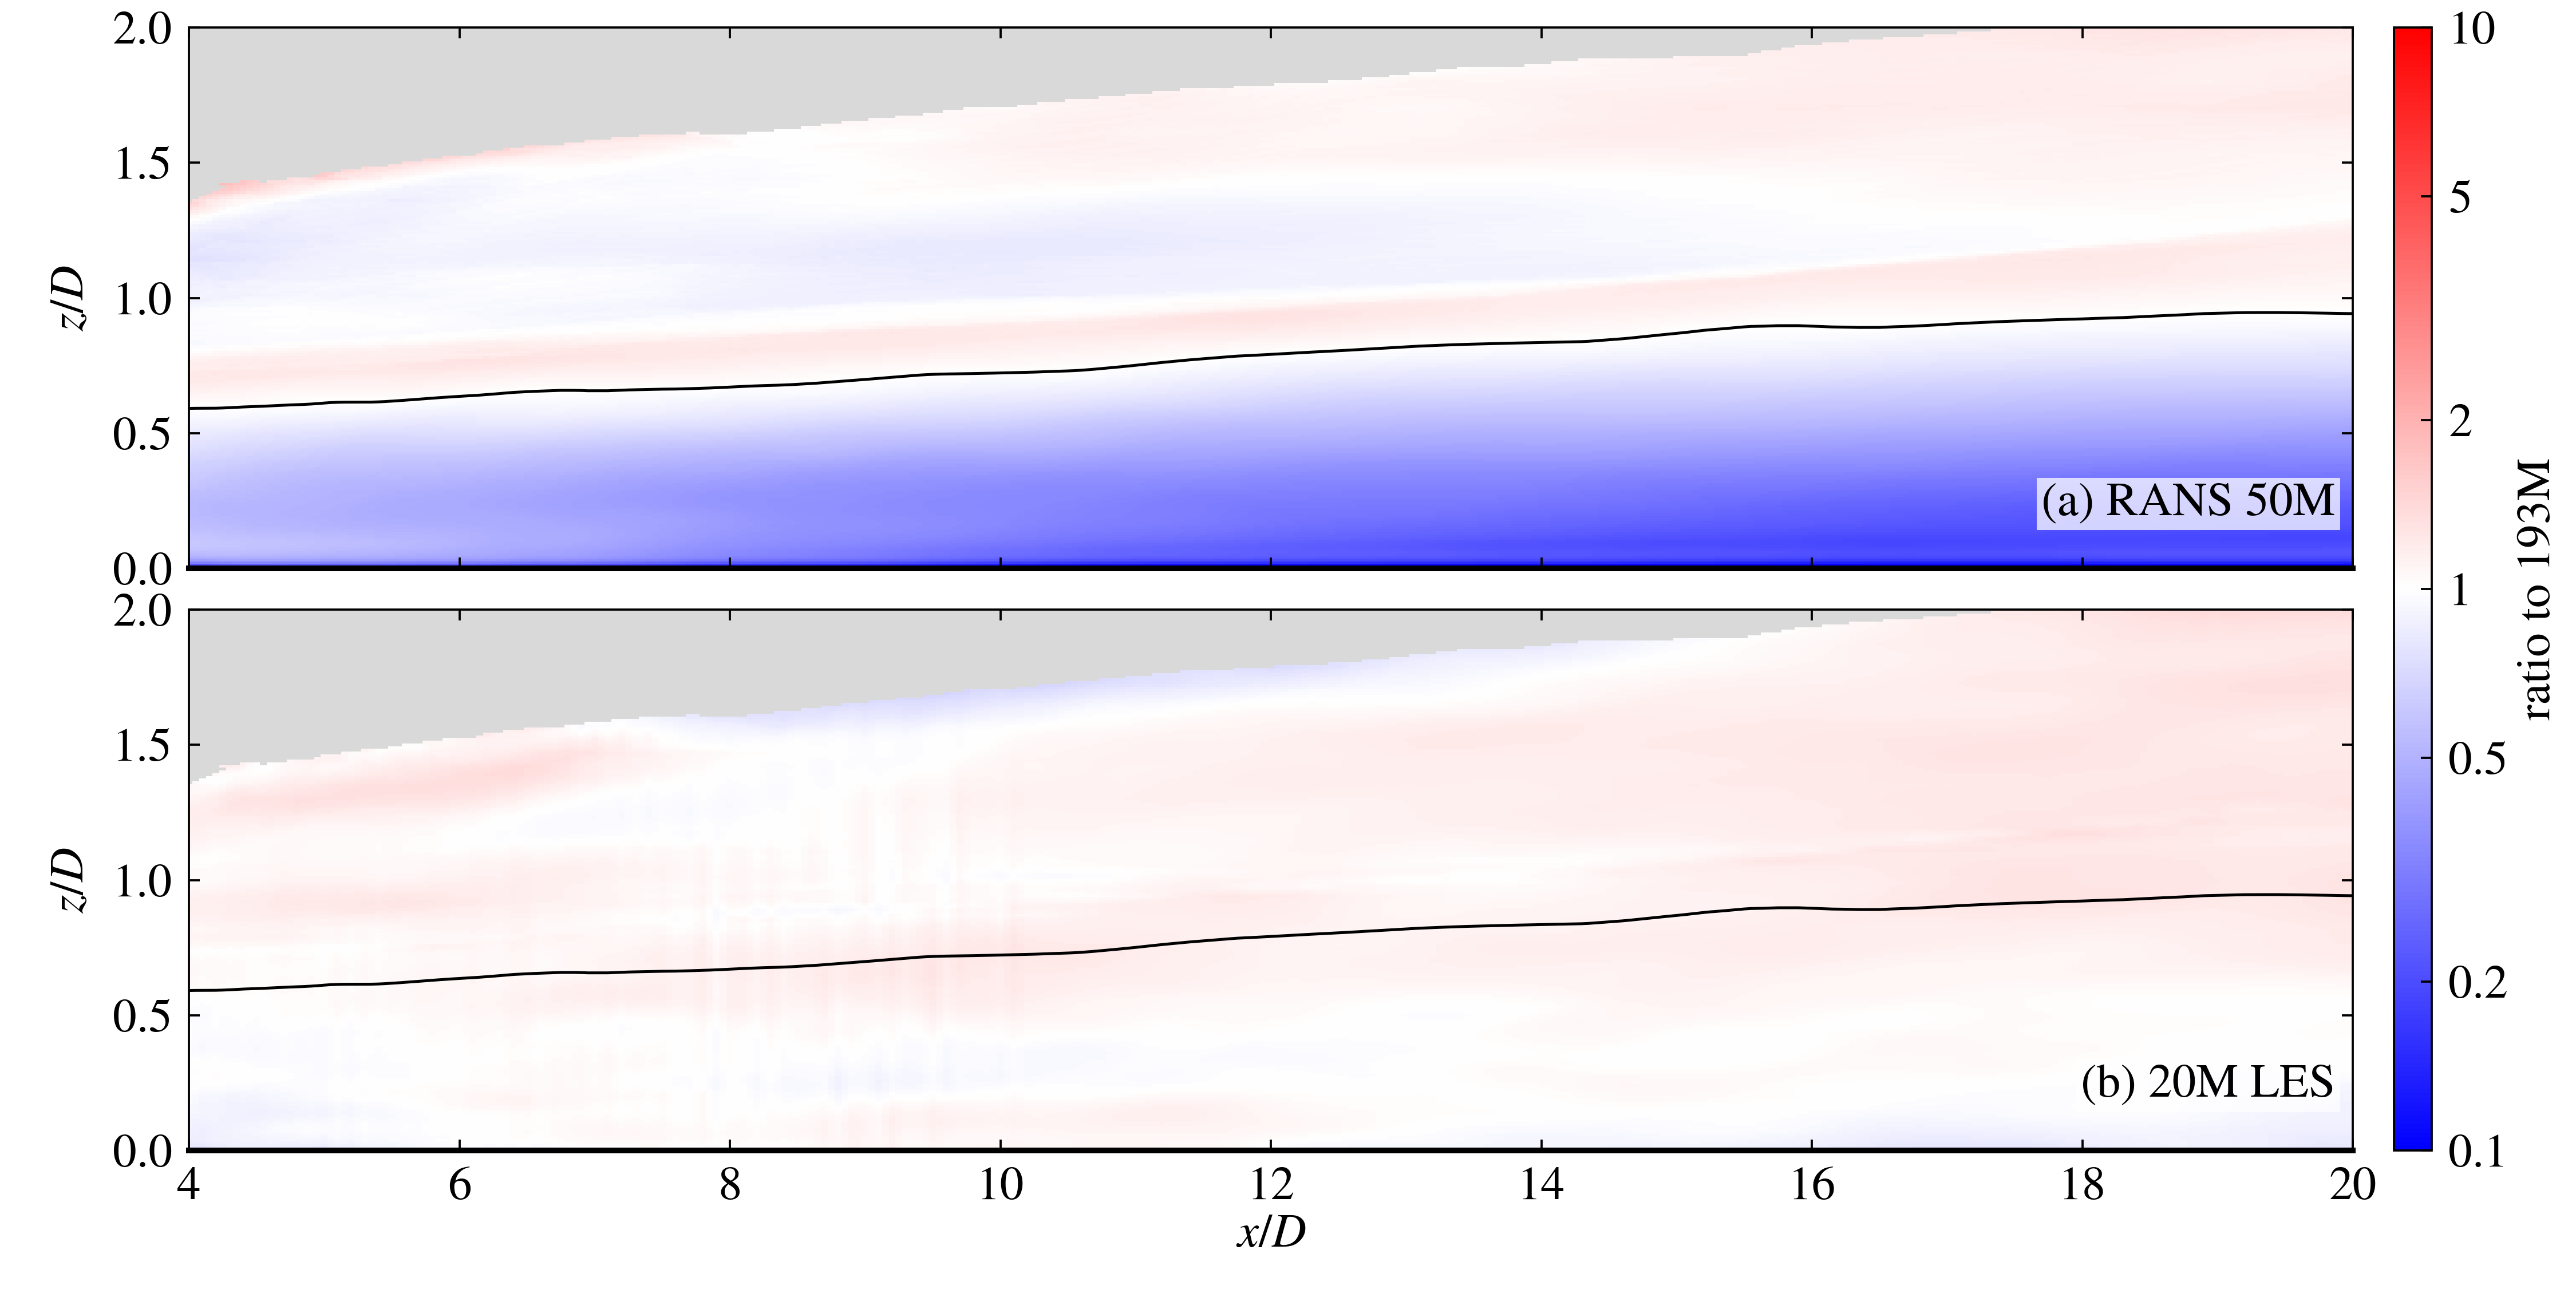
\includegraphics[width=0.42\textwidth]{fig_meff_maps.png}
\caption{Project figures behind the two shifts. Left: \texttt{fig\_flux\_eta.pdf} (manuscript Fig.~6 bottom).
Right: \texttt{fig\_meff\_maps.png} (manuscript Fig.~10), with $z_x(x)$ as the black line; the grey wedge at
$x/D$ 3--4.25 above $z/D\sim1.2$ includes the manual jet-edge mask.}
\end{figure}

\subsection*{E2\quad Where the manuscript says more than the evidence shows}

{\footnotesize
\begin{longtable}{@{}L{4.6cm} L{6.6cm} L{5.4cm}@{}}
\toprule
Sentence (location) & Evidence & Neutral reading \\
\midrule
\endhead
``The RANS thus replaces the missing turbulent transport by a stronger mean upwash, consistent with its stronger
CRVP.'' (4.1, l.\,586) & Flux split measured. Swap test (coord.): RANS velocity alone raises the mean flux 1.2,
2.7, 2.9 times at $x/D$ 5, 10, 20; RANS coolant distribution alone 1.6, 2.7, 2.5 times. Literature: SST
over-predicts CRVP strength (Stratton and Shih; Laroche), $k$--$\varepsilon$ under-predicts (Coletti; Stratton and
Shih); no circulation ratio and no flux split found in 128 stored papers. & The excess mean-flow flux comes in
similar parts from the velocity field and from the coolant sitting where the upwash is; ``replaces'' implies a
cause not tested. ``Consistent with'' is defensible; the mean velocity field, not the CRVP alone, was swapped. \\
``A stronger CRVP with a stronger mean upwash \dots\ keeps the coolant on the centreline and sweeps hot gas under
the flanks.'' (4.1, l.\,597) & Lateral budget (coord.): inward mean sweep 1.2--1.9 times the 193M; RANS outward
turbulent flux 0.4 of the 193M at $x/D$ 5, about equal from $x/D$ 10. & Measured for the flux budget once the
lateral budget is added; attribution to the vortex pair remains an interpretation. \\
``The narrow, steep film of the RANS is thus the result of its weak lateral diffusivity.'' (4.2, l.\,890) & F19
split; lateral budget (coord.) shows the RANS outward turbulent flux equal to the reference from $x/D\sim10$, and
F19b itself gives a total near zero. & Weak diffusivity with steep gradients gives the same flux; the lateral
budget assigns the downstream narrowness to the inward mean sweep. The two sections give different causes. \\
``about half'' / ``several times'' (4.1, l.\,585) & Comment: 0.37--0.61 and 1.65--5.9 on $z_x$. Scratch test at
fixed heights: turbulent RANS/193M 0.67--0.98 at $z/D=1.0$; at $z/D$ 0.25 the RANS turbulent flux is
downward. & The ordering (turbulent $>$ mean in
the 193M, never in the RANS) is robust; the ratio is a property of the chosen surface. \\
``Above $z_x$ \dots\ result of compensating errors.'' (4.2, l.\,777; abstract; C2) & Factor ratios measured
($k^{1/2}$ 1.09--1.16, length 0.71--0.77, $1/\cos\theta$ 1.23--1.32 by slab). & Measured on the strained 32--56\,\%
of the volume. ``Compensating'' is a reading; the memory rule on neutral voice asks for findings without
advocacy, which the sentence meets if it names the factors. \\
``A compensation of this kind above the near-wall layer has not been found described for film cooling.''
(l.\,782) & \texttt{compensating\_errors\_literature.md}: not found in 128 stored PDFs; Acharya 2001 not text-searched;
Schmitt 2007 not stored. & Supportable with its scope: ``in the literature reviewed''. \\
``How closely the mean features of a RANS solution match resolved ones \dots\ has not been reported.''
(l.\,247) & CRVP note: no circulation ratio found; contour comparisons exist (Stratton and Shih; Laroche;
Lakehal). & Too strong as written; qualitative comparisons exist. \\
``No study takes one shaped hole through RANS, LES and DNS on one mesh family.'' (l.\,268) & No search note
covers it. & Not checked from the files. \\
``Hoda and Acharya also reported an over-prediction of the CRVP'' (l.\,599) & Not in the stored literature
note; two stored papers report the opposite sign for $k$--$\varepsilon$. & Cannot be checked here; the model
dependence of the sign should be stated. \\
``RANS eddy viscosity \dots\ is 0.55--0.75 times the reference'' (l.\,766) & Slabs: 0.55--0.66. & Macro value
0.75 not supported. \\
``the 20M LES and the 50M 3DNS lie $\sim$10\,\% above the reference'' (l.\,784) & No file found; plan of record:
within $\pm2$ SE of zero; W1 item 3 due 1 Dec. & Not yet shown. \\
``the 20M curve lies to its right over most of the volume'' (3.3, l.\,447) & Fig.~2: in the near film about
25\,\% of the 20M volume lies above 2, in the far film about 50\,\% (read from the figure). & Contradicts the
figure. \\
Text-only results whose figures were dropped: coherence at St 0.27 (F6), mean $\gamma$ 0.17/0.72 (F9),
misalignment location (F17), $L_{\mathrm{eff}}$ within 7\,\% of the dissipation length (F18), coherent share
(no figure). & Numbers exist in the plan. & Acceptable in a conference paper if each is one sentence; reviewers
cannot see the evidence. \\
\bottomrule
\end{longtable}}

\subsection*{E3\quad Where the plan and the manuscript disagree}

{\footnotesize
\begin{longtable}{@{}L{3.6cm} L{4.3cm} L{4.3cm} L{4.2cm}@{}}
\toprule
Item & Working plan & Manuscript & Data file \\
\midrule
\endhead
Near-wall $\mu$ ratio & 0.55--0.66 & 0.55--0.75 (body), half to two thirds (abstract) & 0.55--0.66 \\
$z_x$ anchor & 0.59 at $x/D$ 4 to 0.94 & 0.62 at $x/D$ 3 to 0.94 & 0.620 (3), 0.591 (4), 0.942 (20) \\
Start of comparison & $x/D$ 3--20 and ``jet ($x/D<4$) left out'' (both in the plan) & $x/D$ 3--20 & -- \\
Scale-resolving $\mu$ & ``about 10\,\% above'' (working); ``within $\pm2$ SE'' (HEAD) & about 10\,\% above &
none found \\
Flux crossover & $x/D\approx5$ (4.5--4.75) & $x/D\sim5$ in text, 4.3 in comment & figure: about 4.3 \\
Resolution figure & five meshes, far film 10--20 & four meshes, far film labelled 10--25 & figure as manuscript \\
Figures & F2, F6, F9, F12, F17, F18 planned & not used & -- \\
Conclusions & empty & four items & -- \\
Mid-pitch $\eta$ 193M at $x/D$ 20 & 0.025 & 0.024 (Table~2, text) & -- \\
Recovered shares, last two runs & empty & 63\,\%, 54\,\% & computed from window means \\
\bottomrule
\end{longtable}}

\subsection*{E4\quad Claims that survived because a figure was redrawn}

\begin{itemize}
\item \textbf{Fig.~10 (eddy-viscosity maps).} A manual grey mask joins $(x/D,z/D)=(3.0,1.15)$ to $(4.25,1.41)$ and
  hides a saturated patch (ratio $\ge3$ in panels c and d); $f_{\min}=0.2$ was chosen as the smallest value that
  removes the saturated top-left patch from panels b--d (\texttt{fig\_meff\_maps.py}, data table). The numbers
  ($z_x$, the split) do not use the mask, and the band means above $z_x$ (0.98--1.03) carry the claim without it.
  The claim survives on the numbers; the caption states only the $f_{\min}$ rule and does not disclose the manual
  mask.
\item \textbf{Far-wall over-prediction.} Removed by re-estimation (3D mask), not by redrawing. The change is
  justified and recorded; the conditional and unconditional $\mu$ maps differ by more than a factor 2.7 in 10\,\%
  of the cells (90th percentile of $|\ln|$ 1.02), so the mask decides the picture above $z_x$.
\item \textbf{Fig.~6 (flux).} Redrawn on the final $z_x$; the qualitative result is unchanged and holds at three
  fixed heights. No claim depends on the redraw.
\end{itemize}

\newpage
%=====================================================================================================
\section*{F\quad Recommendations}

Ordered by effect on the story. Cost: \textbf{cheap} (edit or a short script on data in hand), \textbf{needs a
run} (new extraction on the 193M or RANS fields, or a RANS run). \textbf{[Owner]} marks a decision for the owner.

{\footnotesize
\begin{longtable}{@{}L{0.4cm} L{10.6cm} L{2.4cm} L{2.4cm}@{}}
\toprule
\# & Action & Cost & Decision \\
\midrule
\endhead
1 & Decide how the paper combines the two causes of the narrow film: mean flow (4.1, swap test, lateral budget)
and lateral diffusivity (4.2 step 3, F19). Options: (a) 4.1 states the flux budget and 4.2 the closure input, with
one sentence that links them through the swap test; (b) promote the mean-flow route to a finding and recast 4.2
step 3 as the closure part of it; (c) keep the closure story and move the CRVP flux to a short paragraph. Option (a)
needs the least rewriting and keeps the aims. & cheap & \textbf{[Owner]} \\
2 & Add the swap test and the lateral budget to the plan and to 4.1 (one figure panel or two sentences), then
reword l.\,586 and l.\,597: the excess mean flux comes from both the RANS velocity and the RANS coolant
distribution; attribute to the vortex pair as an interpretation. & cheap (data exist) & -- \\
3 & Reword l.\,890 (``thus the result of its weak lateral diffusivity'') to agree with item 1. & cheap & after 1 \\
4 & Fix the near-wall ratio macro (\texttt{\textbackslash muNearHigh} 0.75 $\to$ 0.66) and align $z_x$ anchors
between plan and manuscript. Confirm that the split layer and the map line use the same $z_x$ file. & cheap & -- \\
5 & State in 4.2 that $z_x$ is defined by the ratio, so the sign below it holds by construction, and give the
masked volume fraction above $z_x$ (32--56\,\%). Disclose the manual jet-edge mask in the caption of Fig.~10, or
remove it and accept the patch. & cheap & \textbf{[Owner]} mask \\
6 & Replace ``about half'' with the ordering statement, or quote the ratio with its surface; add the height
sensitivity (scratch result) as one sentence. The scratch file sits in a temporary folder; copy its script to
\texttt{figures/code/}. & cheap & -- \\
7 & Scale-resolving eddy-viscosity bound (``$\sim$10\,\% above''): hold until W1 item 3 (1 Dec), or remove. &
needs a run (due) & -- \\
8 & Section 3.3: supply the volume fractions above 2 per mesh and region, the wall units, the 5M curve; redraw
Fig.~2 with far film 10--20; correct the 20M sentence. & needs a run (extraction) & -- \\
9 & Abstract and conclusions: carry the same findings. Either add the mean-flow result and the film-only
heat-flux result to the abstract, or drop the mean-flow headline from conclusion 1. & cheap & \textbf{[Owner]} \\
10 & Qualify novelty sentences: l.\,247 (qualitative RANS--resolved comparisons exist), l.\,782 (``in the
literature reviewed''), l.\,268 (needs a search); verify Hoda and Acharya (2000) and state that the sign of the
CRVP error depends on the model. & cheap (search) & -- \\
11 & 4.3: finish $\Pr_t$ 0.4 in the film, resolved stresses alone, $\gamma=1$; until then aims 3 and conclusion 3
stay partial. & needs a run & \textbf{[Owner]} submit without them? \\
12 & Title: ``Resolution Ladder'' names aims 1 and 4; the results now weigh on the closure and the mean flow. &
cheap & \textbf{[Owner]} \\
13 & Length: cut about 1270 words (Figure~\ref{fig:wb}); largest excesses 4.2 (+305), 4.1 (+244), Methods (+202).
If the page count stays above 15, drop the cross-plane figure (Fig.~12) to text. & cheap &
\textbf{[Owner]} figure \\
14 & Close the remaining open markers: literature RANS $\bar\eta$ error (Intro), time integration and flush time
(Methods), discharge coefficients (4.1), far-film wall $\Pr_t$ (4.2, may stay as a stated limit). & cheap to
needs a run & -- \\
\bottomrule
\end{longtable}}

\end{document}
